\documentclass[12pt,a4paper]{report}
\usepackage[utf8]{inputenc}
\usepackage[russian]{babel}
\usepackage[OT1]{fontenc}
\usepackage{amsmath}
\usepackage{amsfonts}
\usepackage{amssymb}
\usepackage{graphicx}
\usepackage{cmap}					% поиск в PDF
\usepackage{mathtext} 				% русские буквы в формулах
%\usepackage{tikz-uml}               % uml диаграммы


% Генератор текста
\usepackage{blindtext}

%------------------------------------------------------------------------------

% Подсветка синтаксиса
\usepackage{color}
\usepackage{xcolor}
\usepackage{listings}
 
 % Цвета для кода
\definecolor{string}{HTML}{B40000} % цвет строк в коде
\definecolor{comment}{HTML}{008000} % цвет комментариев в коде
\definecolor{keyword}{HTML}{1A00FF} % цвет ключевых слов в коде
\definecolor{morecomment}{HTML}{8000FF} % цвет include и других элементов в коде
\definecolor{captiontext}{HTML}{FFFFFF} % цвет текста заголовка в коде
\definecolor{captionbk}{HTML}{999999} % цвет фона заголовка в коде
\definecolor{bk}{HTML}{FFFFFF} % цвет фона в коде
\definecolor{frame}{HTML}{999999} % цвет рамки в коде
\definecolor{brackets}{HTML}{B40000} % цвет скобок в коде
 
 % Настройки отображения кода
\lstset{
language=C, % Язык кода по умолчанию
morekeywords={*,...}, % если хотите добавить ключевые слова, то добавляйте
 % Цвета
keywordstyle=\color{keyword}\ttfamily\bfseries,
stringstyle=\color{string}\ttfamily,
commentstyle=\color{comment}\ttfamily\itshape,
morecomment=[l][\color{morecomment}]{\#}, 
 % Настройки отображения     
breaklines=true, % Перенос длинных строк
basicstyle=\ttfamily\footnotesize, % Шрифт для отображения кода
backgroundcolor=\color{bk}, % Цвет фона кода
%frame=lrb,xleftmargin=\fboxsep,xrightmargin=-\fboxsep, % Рамка, подогнанная к заголовку
frame=tblr
rulecolor=\color{frame}, % Цвет рамки
tabsize=3, % Размер табуляции в пробелах
 % Настройка отображения номеров строк. Если не нужно, то удалите весь блок
numbers=left, % Слева отображаются номера строк
stepnumber=1, % Каждую строку нумеровать
numbersep=5pt, % Отступ от кода 
numberstyle=\small\color{black}, % Стиль написания номеров строк
 % Для отображения русского языка
extendedchars=true,
literate={Ö}{{\"O}}1
  {Ä}{{\"A}}1
  {Ü}{{\"U}}1
  {ß}{{\ss}}1
  {ü}{{\"u}}1
  {ä}{{\"a}}1
  {ö}{{\"o}}1
  {~}{{\textasciitilde}}1
  {а}{{\selectfont\char224}}1
  {б}{{\selectfont\char225}}1
  {в}{{\selectfont\char226}}1
  {г}{{\selectfont\char227}}1
  {д}{{\selectfont\char228}}1
  {е}{{\selectfont\char229}}1
  {ё}{{\"e}}1
  {ж}{{\selectfont\char230}}1
  {з}{{\selectfont\char231}}1
  {и}{{\selectfont\char232}}1
  {й}{{\selectfont\char233}}1
  {к}{{\selectfont\char234}}1
  {л}{{\selectfont\char235}}1
  {м}{{\selectfont\char236}}1
  {н}{{\selectfont\char237}}1
  {о}{{\selectfont\char238}}1
  {п}{{\selectfont\char239}}1
  {р}{{\selectfont\char240}}1
  {с}{{\selectfont\char241}}1
  {т}{{\selectfont\char242}}1
  {у}{{\selectfont\char243}}1
  {ф}{{\selectfont\char244}}1
  {х}{{\selectfont\char245}}1
  {ц}{{\selectfont\char246}}1
  {ч}{{\selectfont\char247}}1
  {ш}{{\selectfont\char248}}1
  {щ}{{\selectfont\char249}}1
  {ъ}{{\selectfont\char250}}1
  {ы}{{\selectfont\char251}}1
  {ь}{{\selectfont\char252}}1
  {э}{{\selectfont\char253}}1
  {ю}{{\selectfont\char254}}1
  {я}{{\selectfont\char255}}1
  {А}{{\selectfont\char192}}1
  {Б}{{\selectfont\char193}}1
  {В}{{\selectfont\char194}}1
  {Г}{{\selectfont\char195}}1
  {Д}{{\selectfont\char196}}1
  {Е}{{\selectfont\char197}}1
  {Ё}{{\"E}}1
  {Ж}{{\selectfont\char198}}1
  {З}{{\selectfont\char199}}1
  {И}{{\selectfont\char200}}1
  {Й}{{\selectfont\char201}}1
  {К}{{\selectfont\char202}}1
  {Л}{{\selectfont\char203}}1
  {М}{{\selectfont\char204}}1
  {Н}{{\selectfont\char205}}1
  {О}{{\selectfont\char206}}1
  {П}{{\selectfont\char207}}1
  {Р}{{\selectfont\char208}}1
  {С}{{\selectfont\char209}}1
  {Т}{{\selectfont\char210}}1
  {У}{{\selectfont\char211}}1
  {Ф}{{\selectfont\char212}}1
  {Х}{{\selectfont\char213}}1
  {Ц}{{\selectfont\char214}}1
  {Ч}{{\selectfont\char215}}1
  {Ш}{{\selectfont\char216}}1
  {Щ}{{\selectfont\char217}}1
  {Ъ}{{\selectfont\char218}}1
  {Ы}{{\selectfont\char219}}1
  {Ь}{{\selectfont\char220}}1
  {Э}{{\selectfont\char221}}1
  {Ю}{{\selectfont\char222}}1
  {Я}{{\selectfont\char223}}1
  {і}{{\selectfont\char105}}1
  {ї}{{\selectfont\char168}}1
  {є}{{\selectfont\char185}}1
  {ґ}{{\selectfont\char160}}1
  {І}{{\selectfont\char73}}1
  {Ї}{{\selectfont\char136}}1
  {Є}{{\selectfont\char153}}1
  {Ґ}{{\selectfont\char128}}1
  {\{}{{{\color{brackets}\{}}}1 % Цвет скобок {
  {\}}{{{\color{brackets}\}}}}1 % Цвет скобок }
}
 
 % Для настройки заголовка кода
\usepackage{caption}
\DeclareCaptionFont{white}{\color{сaptiontext}}
\DeclareCaptionFormat{listing}{\parbox{\linewidth}{\colorbox{сaptionbk}{\parbox{\linewidth}{#1#2#3}}\vskip-4pt}}
\captionsetup[lstlisting]{format=listing,labelfont=white,textfont=white}
\renewcommand{\lstlistingname}{Код} % Переименование Listings в нужное именование структуры


%------------------------------------------------------------------------------

\author{А.~И.~Баратынский}
\title{Сети ЭВМ и телекоммуникации}
\begin{document}
\maketitle
\chapter{Задание}
Разработать приложение-клиент и приложение сервер, обеспечивающие функции обмена файлами.
\section{Функциональные требования}
Серверное приложение должно реализовывать следующие функции:
\begin{enumerate}
\item{Прием файла от клиента}
\item{Передача по запросу от клиента списка файлов текущего каталога}
\item{Прием запросов на передачу файла и передача файла клиенту}
\item{Навигация по системе каталогов}
\item{Обработка запроса на отключение клиента}
\item{Принудительное отключение клиента}
\end{enumerate}

Клиентское приложение должно реализовывать следующие функции:
\begin{enumerate}
\item{Получение от сервера списка файлов каталога}
\item{Операции навигации по системе каталога}
\item{Передача файла серверу}
\item{Прием файла от сервера}
\item{Разрыв соединения}
\item{Обработка ситуации отключения клиента сервером}
\end{enumerate}

\section{Нефункциональные требования}
Серверное приложение:
\begin{enumerate}
\item{Прослушивание определенного порта}
\item{Обработка запросов на подключение по этому порту от клиентов}
\item{Поддержка одновременной работы нескольких клиентов через механизм нитей}
\end{enumerate}
Клиентское приложение должно реализовывать следующие функции:
\begin{enumerate}
\item{Установление соединения с сервером}
\end{enumerate}
\section{Накладываемые ограничения}
\begin{enumerate}
\item{Размер передаваемого файла не должен превышать 1 Гб}
\item{Имя передаваемого файла должно быть не более 30 символов}
\end{enumerate}

\chapter{Реализация для работы по протоколу TCP}
\section{Прикладной протокол}
\label{protocol_tcp}
	Первое сообщение клиента всегда имя пользователя. После этого на клиентской стороне создается каталог данного пользователя (в случае, если каталог уже существует, то клиентское приложение просто переходит в него), и начинается дальнейшее взаимодействие.
Далее, с помощью функции getFirstMessage() сервер определяет, какое сообщение было отправлено клиентом. 
\begin{description}
\item[ls]
При таком сообщении от клиента, сервер посылает список всех доступных файлов в данном каталоге. Клиент определяет, что весь список файлов получен, когда приходит сообщение с символом \&.
\item[get]
При таком сообщении от клиента, сервер ожидает нового сообщения с именем передаваемого файла. Когда такое сообщение получено, происходит передача файла. Клиент определяет, что передача файла закончена, когда приходит сообщение с символом \&.
\item[transfer]
Это передача файла от клиента серверу. Первым передается имя файла, затем его размер. После этого начинается передача.
\item[mkdir]
Создание директории на сервере. Вторым сообщением передается название директории.
\item[cd]
Переход в директорию. Во втором сообщении указывается название директории.
\end{description}
\begin{figure}[!htb]
\centering
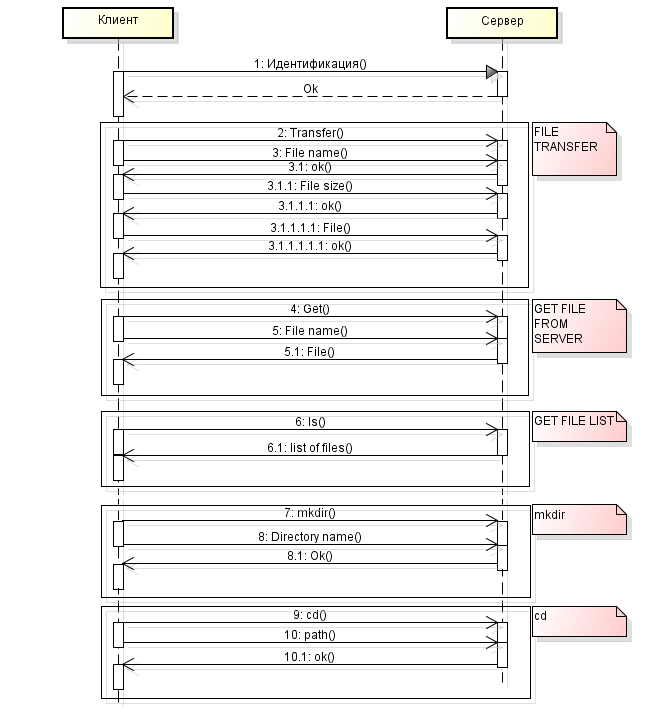
\includegraphics[scale=.7]{seq.eps}
\caption{Sequence diagram}
\label{fig:Sequence diagram}
\end{figure}
\section{Архитектура приложения}
На сервере все файлы хранятся в специальном каталоге SERVER. На клиентской стороне для каждого пользователя создается собственный каталог, в рамках которого он и работает.
\newline
Серверное приложение всегда ждет какого-нибудь сообщения от клиента. После получения сообщения функция getFirstMessage() определяет, какое сообщение было получено. В зависимости от полученного сообщения, сервер вызывает его обработчик.\newline 
Клиентское приложение находится в режиме ожидания ввода очередного сообщения. Если введенное сообщение некорректно (не входит в список известных серверу команд), то клиентское приложение просто игнорирует его.\newline
Несмотря на то, что в протоколе TCP на каждое принятое сервером сообщение по умолчанию посылается подтверждение принятого пакета, мною были добавлены свои ответы сервера. Это сказалось на производительности приложения, т.к. передаваемых пакетов стало в два раза больше, но зато обеспечило легкий переход от TCP к UDP.\newline\newline
\textbf{Формат команд}\newline
В разработанных приложениях один принцип взаимодействия:
сначала от клиента к серверу приходит сообщение с командой, а дальше передаются аргументы команды. Возможно, было бы лучше сделать передачу команды вместе с аргументами в одном пакете, т.к. плюсов в выбранном подходе нет, но такая идея пришла уже после того, как все приложение было написано, поэтому было принято решение оставить все как есть.\newline 
\textbf{transfer}\newline
Сначала посылается команда transfer, затем посылается имя файла, далее посылается размер файла, далее передается тело файла пакетами определенной длины (в данном случае, по 1024 байта). Опять же, передача файлов пакетами определенной длины по протоколу TCP возможно и не самое лучшее решение, т.к. в протоколе TCP передается поток данных, но это было сделано для легкого перехода на протокол UDP, где существуют ограничения на длину пакета. На каждое присланное сообщение сервер отвечает.\newline
\textbf{get}\newline
Все происходит аналогично команде transfer, только в данном случае сообщения идут от сервера клиенту.
\newline
\textbf{cd}\newline
Первым сообщением отсылается сама команда, затем директория, в которую нам нужно перейти.
\newline
\textbf{ls}\newline
Клиент посылает сообщение ls серверу. Сервер обрабатывает сообщение, затем, с помощью системного вызова system("ls>ls"), все файлы текущего каталога записываются в файл ls. Далее сервер считывает из этого файла по одному имени и отправляет его клиенту. После завершения пердачи файл ls удаляется.
\newline
\textbf{mkdir}\newline
Клиент посылает сообщение mkdir. Вторым сообщением он отправляет название новой директории.
\section{Тестирование}
\subsection{Тестовый план и результаты тестирования}
Взаимодействие серверного и клиентского приложений проверялось на одном компьютере. В одном терминале запускался сервер, а в других - клиенты.
\begin{enumerate}
\item{Передача корректного файла серверу}
Передача существующего файла размером меньше 1 Гб завершается без ошибок. 
\item{Передача несуществующего файла серверу}
При попытке передать несуществующий файл серверу выведется сообщение об ошибке: "There is no such file!!!". После этого продолжается обычная работа приложения.
\item{Передача файла размером больше 1 Гб}
При попытке передать файл размером больше 1 Гб серверу выведется сообщение об ошибке: "This file is too big!". После этого продолжается обычная работа приложения. 
\item{Передача файла с помощью команды get}
При вводе команды get, а затем имени нужного файла, происходит его передача от сервера к клиенту.
\item{Ввод команды ls}
После ввода команды ls на клиентску сторону приходит список всех доступных файлов.
\item{Ввод команды cd}
После ввода команды cd и ввода имени каталога происходит переход в это каталог. Тестирование показало, что командой cd можно выйти за переделы каталога SERVER, вплоть до корневой директории. Это несомненный минус данного приложения.
\item{Ввод команды mkdir}
После ввода команды mkdir и ввода имени нового каталога, он создается.
\item{Подключение нескольких клиентов}
Подключение нескольких клиентов проходит успешно. 
В каждом из запущенных клиентов были введены команды transfer, get и ls, на эти команды были получены корректные ответы.
\end{enumerate}

\chapter{Реализация для работы по протоколу UDP}
\section{Прикладной протокол}
Реализация для работы по протоколу UDP не притерпела особых изменений, т.к. изначально, реализация для работы по протоколу TCP была сделана для легкого перехода на протокол UDP.
Первое сообщение клиента всегда имя пользователя. После этого на клиентской стороне создается каталог данного пользователя (в случае, если каталог уже существует, то клиентское приложение просто переходит в него), и начинается дальнейшее взаимодействие.
Далее, с помощью функции getFirstMessage() сервер определяет, какое сообщение было отправлено клиентом. 
\begin{enumerate}
\item{ls}
При таком сообщении от клиента, сервер посылает список всех доступных файлов в данном каталоге. Клиент определяет, что весь список файлов получен, когда приходит сообщение с символом \&.
\item{get}
При таком сообщении от клиента, сервер ожидает нового сообщения с именем передаваемого файла. Когда такое сообщение получено, происходит передача файла. Клиент определяет, что передача файла закончена, когда приходит сообщение с символом \&.
\item{transfer}
Это передача файла от клиента серверу. Первым передается имя файла, затем его размер. После этого начинается передача.
\item{mkdir}
Создание директории на сервере. Вторым сообщением передается название директории.
\item{cd}
Переход в директорию. Во втором сообщении указывается название директории.
\end{enumerate}
\textbf{Объяснение выбранной длины пакета}\newline
	Теоретически, максимальный размер IP-дейтаграммы составляет 65535 байтов, что обусловлено 16-разрядным полем полной длины в IP-заголовке. При размере IP-заголовка 20 байтов и UDP-заголовка - 8 байтов остается максимум 65507 байтов для данных UDP-пакета. Однако в большинстве реализаций устанавливается более жесткое ограничение.
\newline
	Любой хост обязан принимать IP-дейтаграммы длиной по крайней мере 576 байтов. Многие приложения, использующие UDP, спроектированы так, чтобы оперировать данными размером не более 512 байтов, с целью оставаться в гарантированных пределах.
\newline
	В моем приложении, я увеличил минимальный порог в два раза, чтобы немного сократить количество пакетов.
\section{Тестирование}
\subsection{Тестовый план и результаты тестирования}
Взаимодействие серверного и клиентского приложений проверялось на одном компьютере. В одном терминале запускался сервер, а в других - клиенты.
\begin{enumerate}
\item{Передача корректного файла серверу}
Передача существующего файла размером меньше 1 Гб завершается без ошибок. 
\item{Передача несуществующего файла серверу}
При попытке передать несуществующий файл серверу выведется сообщение об ошибке: "There is no such file!!!". После этого продолжается обычная работа приложения.
\item{Передача файла размером больше 1 Гб}
При попытке передать файл размером больше 1 Гб серверу выведется сообщение об ошибке: "This file is too big!". После этого продолжается обычная работа приложения. 
\item{Передача файла с помощью команды get}
При вводе команды get, а затем имени нужного файла, происходит его передача от сервера к клиенту.
\item{Ввод команды ls}
После ввода команды ls на клиентску сторону приходит список всех доступных файлов.
\item{Ввод команды cd}
После ввода команды cd и ввода имени каталога происходит переход в это каталог. Тестирование показало, что командой cd можно выйти за переделы каталога SERVER, вплоть до корневой директории. Это несомненный минус данного приложения.
\item{Ввод команды mkdir}
После ввода команды mkdir и ввода имени нового каталога, он создается.
\item{Подключение нескольких клиентов}
Подключение нескольких клиентов проходит успешно. 
В каждом из запущенных клиентов были введены команды transfer, get и ls, на эти команды были получены корректные ответы.
\end{enumerate}
\chapter{Выводы}
\section{TCP}
  Протокол TCP является сквозным и ориентирован на создание соединений, то есть в данном протоколе создаётся виртуальное соединение. Протокол TCP размещается над сетевым протоколом IP, который даёт возможность TCP посылать и принимать сегменты информации различной длины, вложенные в межсетевые дейтаграммные «конверты» (пакеты).

      При организации связи между парой прикладных процессов протокол TCP обеспечивает следующее: надёжную передачу данных; управление потоком данных; мультиплексирование; организацию, поддержание и сброс виртуального соединения (виртуального канала); приоритетную доставку информации и её безопасность.

      Протокол TCP, в отличие от протокола UDP, создаёт виртуальные соединения или каналы. Подобно модулю UDP, прикладные процессы взаимодействуют с модулем TCP через порты, которые имеют общеизвестные адреса (номера).

Когда прикладной процесс начинает использовать TCP, то этот модуль на хосте и модуль TCP на сервере приложений начинают взаимодействовать. Эти два оконечных модуля, прежде всего, создают виртуальное соединение, которое является дуплексным и расходует ресурсы обоих оконечных модулей TCP. Протокол TCP разбивает поток двоичных разрядов (поступающих с вышележащего уровня) на TCP-сегменты, которые передаются по виртуальному соединению. На приёмном конце производится обратная операция.

      Протокол ТСР требует, чтобы все отправленные сегменты данных были подтверждены с приёмного конца, т.е. используется алгоритм обратной связи. Для повышения эффективности работы используются механизм скользящего окна, тайм-ауты и повторные передачи для обеспечения надёжной доставки. 
\section{UDP}
	Протокол UDP называют протоколом ненадёжной доставки. Этот протокол предоставляет прикладным процессам транспортные услуги, которые немногим отличаются от услуг протокола IP (сетевого уровня).

      Протокол UDP обеспечивает только доставку дейтаграммы и не гарантирует её выполнение. При обнаружении ошибки дейтаграмма просто стирается. Протокол не поддерживает виртуального соединения с удалённым модулем UDP. Чаще всего базируется на принципах динамической маршрутизации (каждая дейтаграмма передаётся по оптимальному маршруту). Основное достоинство — простота.

формат протокола UDP размещается в поле данных IP-пакета (или после заголовка IP-пакета) и содержит следующие поля:

      Поле «Порт источника» (Source Port) указывает порт процесса источника, куда может быть адресован ответ на данное сообщение.

      Поле «Порт получателя» (Destination Port) идентифицирует принимающий процесс.
Под «портом» понимается адрес (номер) некой точки доступа к услугам другого уровня. В случае архитектуры TCP/IP под портом понимается некий номер области памяти, где размещаются передаваемые в сеть (протоколу UDP или TCP) и принимаемые из сети (поступающие в распоряжение операционной системы) данные. Номера портов на передачу и приём в общем случае могут различаться. На приёмной и передающей сторонах взаимодействие процессов в общем случае может происходить через разные номера портов, поэтому указание порта в заголовке UDP-дейтаграммы необходимо.

      В поле «Длина» (Length) указывается размер данной дейтаграммы с учётом длины заголовка в байтах.

      Поле «Контрольная сумма» (Checksum) обеспечивает контроль правильности данных и заголовка. Суммируются все контролируемые 16-битные слова (с циклическим переносом из старшего разряда в младший). Инвертированное значение результата записывается в поле контрольной суммы. Если UDP-дейтаграмма содержит нечетное число байтов, то недостающий последний байт в таких случаях считается нулевым. Этот байт не передается в области данных. 
При подсчете контрольной суммы протокол UDP учитывает 12-байтовый псевдозаголовок (pseudo header). Псевдозаголовок включает в себя: IP-адрес источника, IP-адрес приемника, протокол (код 17) и длину UDP-дейтаграммы.
Если источник проставил контрольную сумму, а адресат при ее проверке обнаружил ошибку, то UDP-дейтаграмма "молчаливо отбрасывается" - не генерируется никакого сообщения об ошибке.\newline
Реализованные приложения работают хорошо, но приложение с использованием протокола UDP работает быстрее. Причины перечислены выше. 
\chapter*{Приложения}
\section*{Описание среды разработки}
Linux debian 3.2.0-4-486 1 Debian 3.2.60-1+deb7u3 i686 GNU/Linux.\newline Среда разработки - Eclipse.\newline
Windows 8.\newline Среда разработки - Visual Studio 2010.

\section*{Листинги}
\subsection*{Linux TCP server}
\lstinputlisting[]
{tcp_serv.c}
\subsection*{Linux TCP client}
\lstinputlisting[]
{tcp_client.c}
\subsection*{Linux UDP server}
\lstinputlisting[]
{udp_serv.c}
\subsection*{Linux UDP client}
\lstinputlisting[]
{udp_client.c}
\subsection*{Windows TCP server}
\lstinputlisting[]
{win_tcp_serv.cpp}
\subsection*{Windows TCP client}
\lstinputlisting[]
{win_tcp_client.cpp}
\subsection*{Windows UDP server}
\lstinputlisting[]
{win_udp_serv.cpp}
\subsection*{Windows UDP client}
\lstinputlisting[]
{win_udp_client.cpp}
\subsection*{Пример файла сборки Makefile}
\lstinputlisting[language=make,label={Makefile}]
{Makefile.txt}
\end{document}